\section{Nichtdeterministische Endliche Automaten}

\subsection{Definitionen}
    \begin{mainbox}{Definition NEA}
        Ein \textbf{nichtdeterministischer endlicher Automat (NEA)} ist ein Quintupel $M = (Q, \Sigma, \delta, q_0, F)$. Dabei ist 
        \begin{enumerate}[label= (\roman*)]
            \item $Q$ eine endliche Menge, \textbf{Zustandsmenge} genannt,
            \item $\Sigma$ ein Alphabet, \textbf{Eingabealphabet} genannt,
            \item $q_0 \in Q$ der \textbf{Anfangszustand},
            \item $F \subseteq Q$ die Menge der \textbf{akzeptierenden Zustände} und 
            \item $\delta$ eine Funktion von $Q \times \Sigma$ nach $\mathcal{P}(Q)$, \textbf{Übergangsfunktion genannt}.
        \end{enumerate}
    \end{mainbox}
    Ein NEA kann zu einem Zustand $q$ und einem gelesenen Zeichen $a$ mehrere oder gar keinen Nachfolgezustand haben.

    \begin{mainbox}{Konfigurationen für NEAs}
		Eine \textbf{Konfiguration} von $M$ ist ein Tupel $(q, w) \in Q \times \Sigma^*$. 
	\end{mainbox}
	\begin{itemize}[label=-]
		\item ''$M$ befindet sich in einer Konfiguration $(q,w) \in Q \times \Sigma^*$, wenn $M$ im Zustand $q$ ist und noch das Suffix $w$ eines Eingabewortes lesen soll.''
		\item Die Konfiguration $(q_0, x) \in \{q_0\} \times \Sigma^*$ ist die \textbf{Startkonfiguration für das Wort $x$}.
	\end{itemize}
	\begin{mainbox}{}
		Ein \textbf{Schritt} von $M$ ist eine Relation (auf Konfigurationen) $\sststile{M}{} \ \subseteq (Q \times \Sigma^*)\times(Q\times \Sigma^*)$, definiert durch
		$$(q, w) \sststile{M}{}(p, x) \iff w = ax, a \in \Sigma \text{ und }p \in \delta(q, a)$$
	\end{mainbox}

	\begin{mainbox}{Berechnungen für NEAs}
		Eine \textbf{Berechnung von $\mathbf{M}$} ist eine endliche Folge $C_1, ..., C_k$ von Konfigurationen, so dass 
		$$C_i \sststile{M}{} C_{i+1} \text{ für alle } 1 \leq i \leq k.$$

		Eine \textbf{Berechnung von $\mathbf{M}$ auf $\mathbf{x}$} ist eine Berechnung $C = C_0, ..., C_m$, wobei $C_0 = (q_0, x)$ und \textbf{entweder} $C_m \in Q \times \{\lambda\}$ \textbf{oder} $C_m = (q, ay)$ für ein $a \in \Sigma, y \in \Sigma^*$ und $q \in Q$, so dass $\delta(q, a) = \emptyset$.
	\end{mainbox}
	Falls $C_m \in F \times \{\lambda\}$, sagen wir, dass $C$ eine \textbf{akzeptierende Berechnung} von $M$ auf $x$ ist, und dass \textbf{$M$ das Wort $x$ akzeptiert}.

   
    Die Relation $\sststile{M}{*}$ ist die reflexive und transitive Hülle von $\sststile{M}{}$, genau wie bei einem EA.

    Wir definieren $$\mathbf{L(M)} = \{w \in \Sigma^* \mid (q_0, w) \sststile{M}{*} (p, \lambda) \text{ für ein } p \in F\}$$ als die \textbf{von $\mathbf{M}$ akzeptierte Sprache.}
    \begin{mainbox}{}
        Zu der Übergangsfunktion $\delta$ definieren wir die Funktion $\hat{\delta}: (Q \times \Sigma^*) \to \mathcal{P}(Q)$ wie folgt:
        \begin{enumerate}[label=(\roman*)]
            \item $\hat{\delta}(q, \lambda) = \{q\}$ für alle $q \in Q$
            \item $\hat{\delta}(q, wa) = \bigcup_{r \in \hat{\delta}(q,w)}\delta(r,a)$ für alle $q\in Q, a \in \Sigma, w \in \Sigma^*$.
        \end{enumerate}
    \end{mainbox}

    
    \myTitle{Repetition Pumping Lemma - Aufgabe mit Case Distinction (12.b)}

        Wir zeigen per Pumping Lemma, dass die Sprache 
        $$L = \{w \in \{a, b, c\}^* \mid w \text{ enthält das Teilwort $ab$ gleich oft wie das Teilwort $ba$}\}$$
        nicht regulär ist.
    

        Zur Erinnerung:
        \begin{mainbox}{Pumping Lemma}
            Sei $L$ regulär. Dann existiert eine Konstante $n_0 \in \N$, so dass jedes Wort $w \in \Sigma^*$ mit $|w| \geq n_0$ in drei Teile $x, y$ und $z$ zerlegen lässt, das heisst $w = yxz$, wobei
            \begin{enumerate}[label=(\roman*)]
                \item $|yx| \leq n_0$
                \item $|x| \geq 1$
                \item entweder $\{yx^kz \mid k \in \N\} \subseteq L$ oder $\{yx^kz \mid k \in \N\} \cap L = \emptyset$.
            \end{enumerate}
        \end{mainbox}
    
        \textbf{Lösung}
    
        Sei $L$ regulär. 
        
        Nach dem Pumping Lemma existiert eine Konstante $n_0 \in \N$, so dass jedes Wort $w$ mit $|w| \geq n_0$ die Bedingung des PL erfüllt.
        
        Sei $w = (abc)^{n_0}(bac)^{n_0}$. Offensichtlich gilt $|w| \geq n_0$. Nach dem PL existiert eine Zerlegung $w = yxz$, die (i), (ii) und (iii) erfüllt.
        
        Da $yxz$ die Bedingung (i) erfüllt, gilt $|yx| \leq n_0$. Insbesondere folgt daraus, dass $x$ komplett in der ersten Hälfte (i.e. $(abc)^{n_0}$) enthalten ist.
    
        Aus (ii) folgt weiter, dass $x$ mindestens ein Buchstaben enthält.
    
        \textbf{Case Distinction}
        \begin{enumerate}[label=\Roman*.]
            \item \textbf{Case $\mathbf{x = c}$}
            
            In diesem Fall enthält $yx^0z = yz$ das Teilwort $ba$ einmal mehr als $ab$. 
    
            Somit gilt in diesem Fall $yx^0z \notin L$.
            
            \item \textbf{Case $\mathbf{x}$ enthält mindestens ein $\mathbf{a}$ oder $\mathbf{b}$}
            
            Wir betrachten $yx^0z = yz$. 
            In diesem Fall bleibt die Anzahl der Teilwörter $ba$ gleich oder erhöht sich. 
            Da aber die Anzahl der Teilwörter $ab$ um mindestens $1$ kleiner wird, gilt $yx^0z \notin L$.
        \end{enumerate}
        
        Da die Case Distinction alle Fälle abdeckt folgt für die Zerlegung $yx^0z \notin L$. Aus $yxz \in L$ ergibt sich somit ein Widerspruch. 
    
        Demnach ist die Annahme falsch und $L$ nicht regulär.
    
        $\hfill\blacksquare$
    
        
        \pagebreak
    
        \myTitle{NEA - Beispiel aus der Vorlesung}
        
        Wir betrachten folgenden NEA $M = (\{q_0,q_1,q_2\}, \Sigma_{\text{bool}}, \delta, q_0, \{q_2\})$
        \begin{figure}[htp]
            \centering
            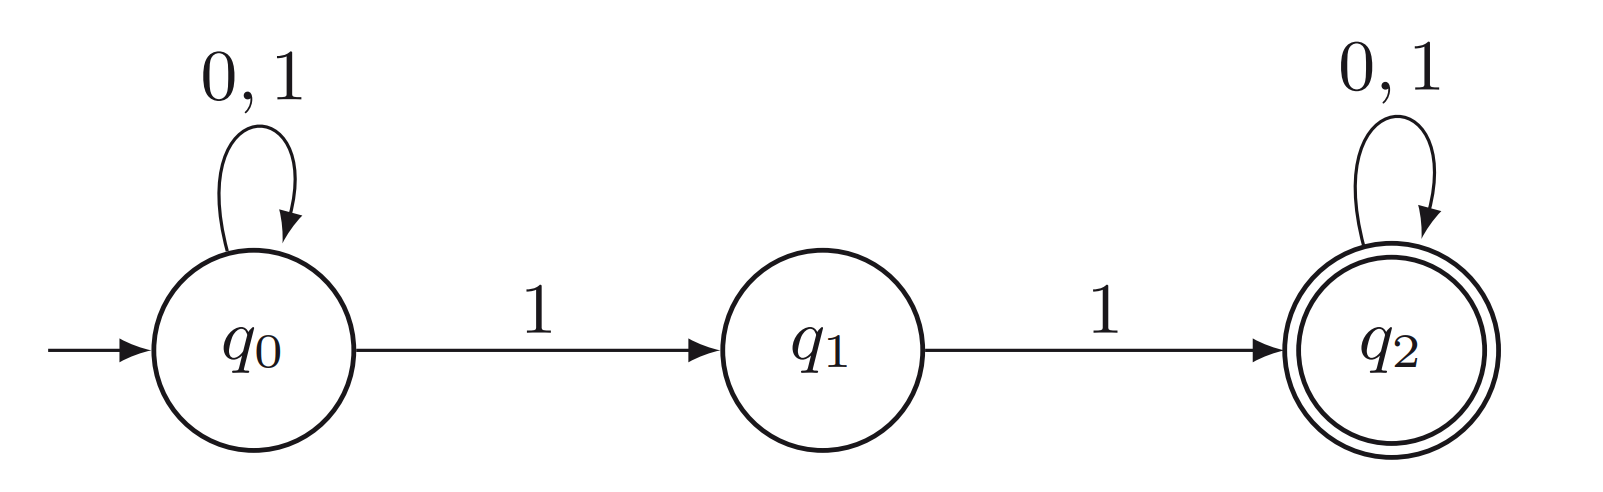
\includegraphics[width=0.8\textwidth]{Images/Beispiel_NEA.png}
            \caption[]{Abb. 3.15 aus dem Buch}
        \end{figure}
    
        \myTitle{Berechnungsbaum}

        Für ein Wort $x \in (\Sigma_{\text{bool}})^*$ ist ein Berechnungsbaum $\mathbf{\mathcal{B}_M(x)}$ nützlich, um zu erkennen, ob  $x \in L(M)$.
    
        \begin{figure}[htp]
            \centering
            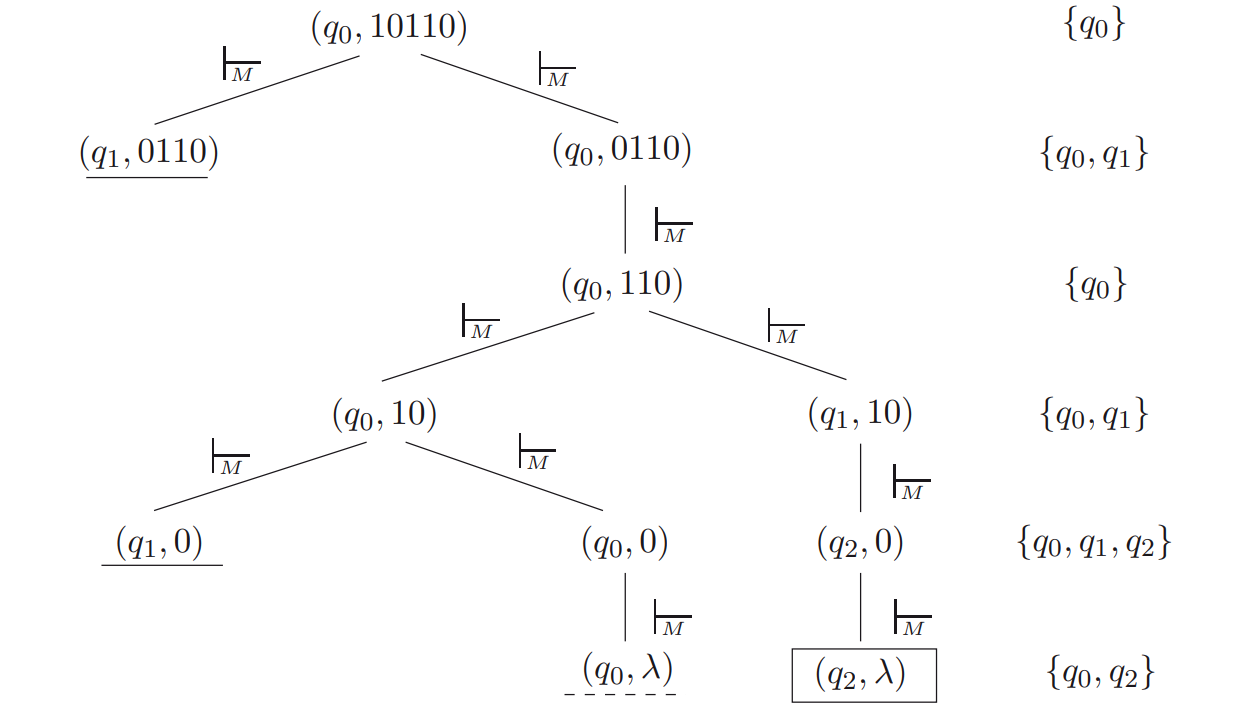
\includegraphics[width=0.6\textwidth]{Images/Berechnungsbaum.png}
            \caption{Abb. 3.16 aus dem Buch}
        \end{figure}
    
        Wir können die Sprache des NEA bestimmen.
        \begin{subbox}{Lemma 3.5}
            $$L(M) = \{x11y \mid x,y \in (\Sigma_{\text{bool}})^*\}$$
        \end{subbox}
        \textbf{Beweisidee}
    
        Beide Inklusionen zeigen und fertig. (Siehe Buch)
    
        Wir definieren die Klasse $\mathbf{\mathcal{L}_{\text{NEA}}}$.
        \begin{mainbox}{}
            $$\mathbf{\mathcal{L}_{\text{NEA}}} = \{L(M) \mid M \text{ ist ein NEA}\}$$
        \end{mainbox}
    
    
    
        \subsection{Äquivalenz von NEA und EA}
        Beweis von $\mathbf{\mathcal{L}_{\text{NEA}}} = \mathbf{\mathcal{L}_{\text{EA}}}$ per \textbf{Potenzmengenkonstruktion}.
        \begin{mainbox}{Satz 3.2}
            Zu jedem NEA $M$ existiert ein EA $A$, so dass
            $$L(M) = L(A)$$
        \end{mainbox}
        \textbf{Beweisidee}
    
        Potenzmengenkonstruktion und dann Induktion auf der Länge von einem Input i.e. $|x|$. (Siehe Buch)
    
    
    
        \textbf{Potenzmengenkonstruktion}
        \begin{subbox}{}
            Sei $M = (Q, \Sigma, \delta_M, q_0, F)$ ein NEA. Wir konstrurieren einen äquivalenten Endlichen Automaten $A = (Q_A, \Sigma_A, \delta_A, q_{0A}, F_A)$.
            \begin{enumerate}[label = (\roman*)]
                \item $Q_A = \{\langle P \rangle \mid P \subseteq Q\}$
                \item $\Sigma_A = \Sigma$
                \item $q_{0A} = \langle\{q_0\}\rangle$
                \item $F_A = \{\langle P\rangle \mid P \subseteq Q \text{ und } P \cap F \neq \emptyset\}$
                \item $\delta_A: (Q_A \times \Sigma_A) \to Q_A$ ist eine Funktion, definiert wie folgt. Für  jedes $\langle P \rangle \in Q_A$ und jedes $a \in \Sigma_A$ ist 
                \begin{align*}
                    \delta_A(\langle P \rangle, a) &= \left\langle \bigcup_{p \in P} \delta_M(p, a) \right\rangle\\
                    &= \left\langle\{q \in Q \mid \exists p \in P, \text{ so dass }q \in \delta_{M}(p, a)\}\right\rangle
                \end{align*}
            \end{enumerate}
        \end{subbox}
    
        \begin{figure}[htp]
            \centering
            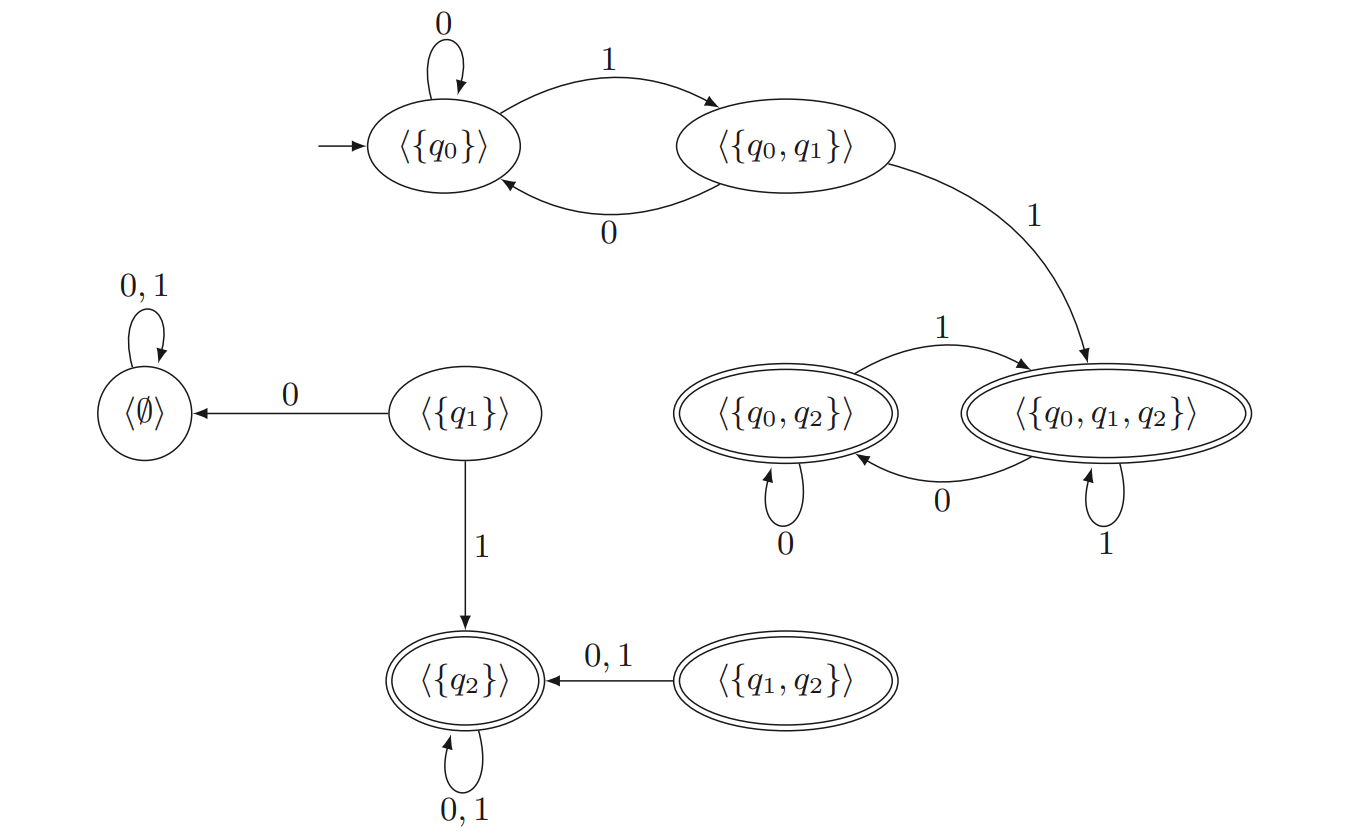
\includegraphics[width=0.75\textwidth]{Images/Potenzmengenkonstruktion_Beispiel.png}
            \caption{Abb. 3.18 im Buch}
        \end{figure}
    
    
    
        \subsection{Exponentiell mehr Zustände - manchmal}
        Sei 
        $$L_k = \{x1y \mid x \in (\Sigma_{\text{bool}})^*, \ y \in (\Sigma_{\text{bool}})^{k-1}\}$$
        Folgender NEA $A_k$ mit $k+1$ akzeptiert $L_k$.
        \begin{figure}
            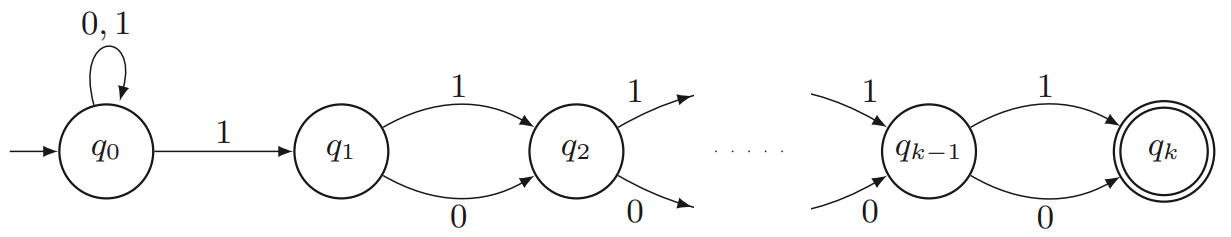
\includegraphics[width=0.8\textwidth]{Images/NEA_A_k.png}
            \caption{Abb. 3.19 im Buch}
        \end{figure}
    
        \begin{mainbox}{Lemma 3.6}
            Für alle $k \in \N \setminus \{0\}$ muss jeder EA, der $L_k$ akzeptiert, mindestens $2^k$ Zustände haben.
        \end{mainbox}
        \textbf{Beweis}
    
        Sei $B_k = (Q_k, \Sigma_{bool}, \delta_k, q_{0k}, F_k)$ ein EA mit $L(B_k) = L_k$. 
        
        Nach \textbf{Lemma 3.3} gilt für $x,y \in (\Sigma_{bool})^*$:
    
        Wenn $\hat{\delta}_k (q_{0k}, x) = \hat{\delta}_k (q_{0k}, y)$, dann gilt für alle $z \in (\Sigma_{bool})^*$:
        $$xz \in L(B_k) \iff yz \in L(B_k)$$
    
        Die Idee des Beweises ist es, eine Menge $S_k$ von Wörtern zu finden, so dass für keine zwei unterschiedlichen Wörter $x, y \in S_k$ die Gleichung $\hat{\delta}_k (q_{0k}, x) = \hat{\delta}_k (q_{0k}, y)$ gelten darf. 
        Dann müsste $B_k$ mindestens $|S_k|$ viele Zustände haben.
        
    
        Wir wählen $S_k = (\Sigma_{bool})^k$ und zeigen, dass $\hat{\delta}_k(q_{0k}, u)$ paarweise unterschiedliche Zustände für alle $u \in  S_k$ sind. 
    
        Wir beweisen dies per Widerspruch. 
    
        Seien $x = x_1x_2...x_k$ und $y = y_1y_2...y_k$ für $x_i,y_i \in \Sigma_{bool}, i \in \{1, ..., k\}$ zwei unterschiedliche Wörter aus $S_k$.
    
        Nehmen wir zum Widerspruch an, dass $\hat{\delta}_k(q_{0k}, x) = \hat{\delta}_k(q_{0k}, y)$.
        
    
        Weil $x \neq y$, existiert ein $j \in \{1, ...,k\}$, so dass $x_j \neq y_j$. O.B.d.A. setzen wir $x_j = 1$ und $y_j = 0$. 
        Betrachten wir nun $z = 0^{j-1}$.  Dann ist 
    
        $xz = x_1...x_{j-1}1x_{j+1}...x_k0^{j-1}$ und $yz = y_1...y_{j-1}0y_{j+1}...y_k0^{j-1}$
    
        und daher $xz \in L_k$ und $yz \notin L_k$. 
        
        Dies ist ein Widerspruch! Folglich gilt $\hat{\delta}_k(q_{0k}, x) \neq \hat{\delta}_k(q_{0k}, y)$ für alle paarweise unterschiedliche $x,y \in S_k = (\Sigma_{bool})^k$.
        
        Daher hat $B_k$ mindestens $|S_k| = 2^k$ viele Zustände.
        
        \hspace*{0pt}\hfill$\blacksquare$
    
    
    \subsection{Mindestanzahl Zustände}
    
        Die Grundidee ist es $n$ Wörter anzugeben und zu beweisen, dass jedes von diesen $n$ Wörtern in einem eigenen Zustand enden muss.
        
        Seien $w_1, ...,w_n$ diese Wörter. Dann geben wir für jedes Paar von Wörtern $w_i \neq w_j$ einen Suffix $z_{i,j}$ an, so dass folgendes gilt:
        $$w_iz_{i,j} \in L \centernot{\iff} w_jz_{i,j} \in L$$
        Dann folgt aus Lemma 3.3
        $$\hat{\delta}(q_0, w_i) \neq \hat{\delta}(q_0, w_j)$$
        
        Es eignet sich die Suffixe als Tabelle anzugeben.
    
        Um die Wörter und Suffixe zu finden, kann es sich als nützlich erweisen, den Endlichen Automaten zu konstruieren.
    
    
    
        \myTitle{Beweisschema}

        Wir nehmen zum Widerspruch an, dass es einen EA für $L$ gibt mit weniger als $n$ Zuständen.
    
        Betrachten wir $w_1, ...,w_n$. Per Pigeonhole-Principle existiert $i < j$, so dass
        $$\hat{\delta}(q_0, w_i) = \hat{\delta}(q_0, w_j)$$
        Per Lemma 3.3 folgt daraus, dass 
        $$\forall z \in \Sigma^*: w_iz \in L \iff w_jz \in L$$
        Für $z = z_{i,j}$ gilt aber per Tabelle $$w_iz_{i,j} \in L \centernot{\iff} w_jz_{i,j} \in L \quad \mathbf{(1)}$$ für alle $i< j$. 
        
        Da keines der $n$ Wörter im gleichen Zustand enden kann, ergibt sich ein Widerspruch.
    
        Dann noch Angabe der Tabelle für $\mathbf{(1)}$
        \begin{table}
            \centering
            \begin{tabular}{c|ccc}
                & $w_2$ & $...$ & $w_n$\\
                \hline
                $w_1$& $z_{1,2}$& ...&$z_{1,n}$\\
                $...$&  & $...$&$...$\\
                $w_{n-1}$& &  & $z_{n-1, n}$
            \end{tabular}
        \end{table}
        \begin{itemize}[label=-]
            \item Wenn es offensichtlich ist, muss $\mathbf{(1)}$ nicht bei jedem Suffix begründet werden.
            \item Ein minimaler endlicher Automat ist nicht notwendig für den Beweis. Hilft aber fürs
            \begin{enumerate}[label=\roman*.]
                \item Finden der $w_i$
                \item Finden der $z_{i, j}$
                \item Beweis von $w_iz_{i,j} \in L \centernot{\iff} w_jz_{i,j} \in L$ (Leicht überprüfbar)
            \end{enumerate}
        \end{itemize}
    
    
    
        \myTitle{Klassische Aufgabe - HS19 Aufgabe 3.a}

        Wir betrachten die Sprache 
        $$L = \{x00y \mid x \in \{0, 1\}^* \text{ und } y \in \{0,1\}\}$$
       
        Konstruieren Sie einen nichtdeterminstischen endlichen Automaten mit höchstens $4$ Zuständen, der $L$ akzeptiert.
        
        \begin{tikzpicture}[shorten >=2pt,node distance=3.5cm,on grid,auto]
            \node[state,initial]    (q_0) {$q_0$};
            \node[state]            (q_1)  [right of=q_0] {$q_1$};
            \node[state]            (q_2)  [right of=q_1] {$q_2$};
            \node[state, accepting] (q_3)  [right of=q_2]    {$q_3$};
            \path[->]
            (q_0) edge [loop above] node {$0, 1$}   (   )
                  edge [bend left]  node {$0$}   (q_1)
            (q_1) edge [bend left]  node {$0$}   (q_2)
            (q_2) edge [bend left] node {$0, 1$}   (q_3)
            ;
        \end{tikzpicture}
    
    
    
        \myTitle{Klassische Aufgabe - HS19 Aufgabe 3.b}

        Zeigen Sie, dass jeder deterministische endliche Automat, der $L$ akzeptiert, mindestens $5$ Zustände braucht.
        
        
        Wir zeichnen den zugehörigen EA zuerst.

        \begin{tikzpicture}[shorten >=2pt,node distance=3cm,on grid,auto]
            \node[state,initial]    (q_0) {$q_0$};
            \node[state]            (q_1)  [right of=q_0] {$q_1$};
            \node[state]            (q_2)  [right of=q_1] {$q_2$};
            \node[state, accepting] (q_3)  [above right of=q_2]    {$q_3$};
            \node[state, accepting] (q_4) [below right of=q_2] {$q_4$};
            \path[->]
            (q_0) edge [loop above] node {$1$}   (   )
                  edge [bend left]  node {$0$}   (q_1)
            (q_1) edge [bend left]  node {$0$}   (q_2)
                  edge [bend left]  node {$1$}   (q_0)
            (q_2) edge [bend left]  node {$0$}   (q_3)
                  edge [bend right] node {$1$}   (q_4)
            (q_3) edge [loop right] node {$0$}   (   )
                  edge [bend left] node {$1$}   (q_4)
            (q_4) edge [bend left]  node {$0$}   (q_1)
                  edge [bend left]  node {$1$}   (q_0)   
            ;
        \end{tikzpicture}
    
        Nehmen wir zum Widerspruch an, dass es einen endlichen Automaten gibt, der $L$ akzeptiert und weniger als $4$ Zustände hat.
    
        Wir wählen die Wörter $B = \{\lambda, 0, 00, 000, 001\}$.
    
        Nach dem Pigeonhole-Principle existieren zwei Wörter $w_i, w_j \in B, w_i \neq w_j$, so dass 
        $$\hat{\delta}(q_0, w_i) = \hat{\delta}(q_0, w_j)$$
        Per Lemma 3.3 folgt daraus, dass 
        $$\forall z \in \Sigma^*: w_iz \in L \iff w_jz \in L$$
        
        Wir betrachten folgende Tabelle mit Suffixen.
        \begin{table}[htp]
            \centering
            \begin{tabular}{c|cccc}
                          & $0$  & $00$& $000$     & $001$    \\
                \hline
                $\lambda$ & $01$ & $1$ & $\lambda$ & $\lambda$\\
                $0$       &      & $1$ & $\lambda$ & $\lambda$\\
                $00$      &      &     & $\lambda$ & $\lambda$ \\
                $000$     &      &     &           & $1$ 
            \end{tabular}
        \end{table}
        Der zeigt für jedes Wortpaar $x, y \in B, x \neq y$ die Existenz eines Suffixes $z$, so dass 
        $$\left(xz \in L \land yz \notin L\right) \lor \left(xz \notin L \land yz \in L\right)$$
        Dies kann man mit den angegebenen Suffixen und dem angegebenen EA einfach überprüfen.
    
        Dies widerspricht der vorigen Aussage, dass ein Wortpaar $w_i, w_j \in B, w_i \neq w_j$ existiert, so dass
        $$\forall z \in \Sigma^*: w_iz \in L \iff w_jz \in L$$
        Somit ist unsere Annahme falsch und ein EA für $L$ muss mindestens $4$ Zustände haben.
    
        $\hfill\blacksquare$
    
        \textbf{Bemerkung}

        Manchmal ist es zu schwierig einen minimalen EA zu finden und es funktioniert einfacher die Wörter durch Trial and Error zu finden. (Siehe Midterm HS22)
    
    
    